\documentclass[a4paper, 12pt]{article}
\usepackage[utf8]{inputenc}
\usepackage[english, ukrainian]{babel}

\usepackage{amsmath, amssymb}
\usepackage{multicol}
\usepackage{graphicx}
\usepackage{float}

\allowdisplaybreaks
\setlength\parindent{0pt}
\numberwithin{equation}{subsection}

\usepackage{hyperref}
\hypersetup{unicode=true,colorlinks=true,linktoc=all,linkcolor=red}

\numberwithin{equation}{subsection}

\renewcommand{\bf}[1]{\textbf{#1}}
\renewcommand{\it}[1]{\textit{#1}}
\newcommand{\bb}[1]{\mathbb{#1}}
\renewcommand{\cal}[1]{\mathcal{#1}}

\renewcommand{\epsilon}{\varepsilon}
\renewcommand{\phi}{\varphi}

\DeclareMathOperator{\diam}{diam}
\DeclareMathOperator{\rang}{rang}
\DeclareMathOperator{\const}{const}

\newenvironment{system}{%
  \begin{equation}%
    \left\{%
      \begin{aligned}%
}{%
      \end{aligned}%
    \right.%
  \end{equation}%
}
\newenvironment{system*}{%
  \begin{equation*}%
    \left\{%
      \begin{aligned}%
}{%
      \end{aligned}%
    \right.%
  \end{equation*}%
}

\makeatletter
\newcommand*{\relrelbarsep}{.386ex}
\newcommand*{\relrelbar}{%
  \mathrel{%
    \mathpalette\@relrelbar\relrelbarsep%
  }%
}
\newcommand*{\@relrelbar}[2]{%
  \raise#2\hbox to 0pt{$\m@th#1\relbar$\hss}%
  \lower#2\hbox{$\m@th#1\relbar$}%
}
\providecommand*{\rightrightarrowsfill@}{%
  \arrowfill@\relrelbar\relrelbar\rightrightarrows%
}
\providecommand*{\leftleftarrowsfill@}{%
  \arrowfill@\leftleftarrows\relrelbar\relrelbar%
}
\providecommand*{\xrightrightarrows}[2][]{%
  \ext@arrow 0359\rightrightarrowsfill@{#1}{#2}%
}
\providecommand*{\xleftleftarrows}[2][]{%
  \ext@arrow 3095\leftleftarrowsfill@{#1}{#2}%
}
\makeatother

\newcommand{\NN}{\mathbb{N}}
\newcommand{\ZZ}{\mathbb{Z}}
\newcommand{\QQ}{\mathbb{Q}}
\newcommand{\RR}{\mathbb{R}}
\newcommand{\CC}{\mathbb{C}}

\newcommand{\Max}{\displaystyle\max\limits}
\newcommand{\Sup}{\displaystyle\sup\limits}
\newcommand{\Sum}{\displaystyle\sum\limits}
\newcommand{\Int}{\displaystyle\int\limits}
\newcommand{\Iint}{\displaystyle\iint\limits}
\newcommand{\Lim}{\displaystyle\lim\limits}

\newcommand*\diff{\mathop{}\!\mathrm{d}}

\newcommand*\rfrac[2]{{}^{#1}\!/_{\!#2}}


\title{{\Huge МАТЕМАТИЧНА ФІЗИКА}}
\author{Скибицький Нікіта}
\date{\today}

\usepackage{amsthm}
\usepackage[dvipsnames]{xcolor}
\usepackage{thmtools}
\usepackage[framemethod=TikZ]{mdframed}

\theoremstyle{definition}
\mdfdefinestyle{mdbluebox}{%
	roundcorner = 10pt,
	linewidth=1pt,
	skipabove=12pt,
	innerbottommargin=9pt,
	skipbelow=2pt,
	nobreak=true,
	linecolor=blue,
	backgroundcolor=TealBlue!5,
}
\declaretheoremstyle[
	headfont=\sffamily\bfseries\color{MidnightBlue},
	mdframed={style=mdbluebox},
	headpunct={\\[3pt]},
	postheadspace={0pt}
]{thmbluebox}

\mdfdefinestyle{mdredbox}{%
	linewidth=0.5pt,
	skipabove=12pt,
	frametitleaboveskip=5pt,
	frametitlebelowskip=0pt,
	skipbelow=2pt,
	frametitlefont=\bfseries,
	innertopmargin=4pt,
	innerbottommargin=8pt,
	nobreak=true,
	linecolor=RawSienna,
	backgroundcolor=Salmon!5,
}
\declaretheoremstyle[
	headfont=\bfseries\color{RawSienna},
	mdframed={style=mdredbox},
	headpunct={\\[3pt]},
	postheadspace={0pt},
]{thmredbox}

\declaretheorem[style=thmbluebox,name=Теорема,numberwithin=subsubsection]{theorem}
\declaretheorem[style=thmbluebox,name=Лема,numberwithin=subsubsection]{lemma}
\declaretheorem[style=thmbluebox,name=Твердження,numberwithin=subsubsection]{proposition}
\declaretheorem[style=thmbluebox,name=Принцип,numberwithin=subsubsection]{th_principle}
\declaretheorem[style=thmbluebox,name=Закон,numberwithin=subsubsection]{law}
\declaretheorem[style=thmbluebox,name=Закон,numbered=no]{law*}
\declaretheorem[style=thmbluebox,name=Формула,numberwithin=subsubsection]{th_formula}
\declaretheorem[style=thmbluebox,name=Рівняння,numberwithin=subsubsection]{th_equation}
\declaretheorem[style=thmbluebox,name=Умова,numberwithin=subsubsection]{th_condition}
\declaretheorem[style=thmbluebox,name=Наслідок,numberwithin=subsubsection]{corollary}

\declaretheorem[style=thmredbox,name=Приклад,numberwithin=subsubsection]{example}
\declaretheorem[style=thmredbox,name=Приклади,sibling=example]{examples}

\declaretheorem[style=thmredbox,name=Властивість,numberwithin=subsubsection]{property}
\declaretheorem[style=thmredbox,name=Властивості,sibling=property]{properties}

\mdfdefinestyle{mdgreenbox}{%
	skipabove=8pt,
	linewidth=2pt,
	rightline=false,
	leftline=true,
	topline=false,
	bottomline=false,
	linecolor=ForestGreen,
	backgroundcolor=ForestGreen!5,
}
\declaretheoremstyle[
	headfont=\bfseries\sffamily\color{ForestGreen!70!black},
	bodyfont=\normalfont,
	spaceabove=2pt,
	spacebelow=1pt,
	mdframed={style=mdgreenbox},
	headpunct={ --- },
]{thmgreenbox}

\mdfdefinestyle{mdblackbox}{%
	skipabove=8pt,
	linewidth=3pt,
	rightline=false,
	leftline=true,
	topline=false,
	bottomline=false,
	linecolor=black,
	backgroundcolor=RedViolet!5!gray!5,
}
\declaretheoremstyle[
	headfont=\bfseries,
	bodyfont=\normalfont\small,
	spaceabove=0pt,
	spacebelow=0pt,
	mdframed={style=mdblackbox}
]{thmblackbox}

\declaretheorem[name=Вправа,numberwithin=subsubsection,style=thmblackbox]{exercise}
\declaretheorem[name=Зауваження,numberwithin=subsubsection,style=thmgreenbox]{remark}
\declaretheorem[name=Визначення,numberwithin=subsubsection,style=thmblackbox]{definition}

\newtheorem{problem}{Задача}[subsection]
\newtheorem{sproblem}[problem]{Задача}
\newtheorem{dproblem}[problem]{Задача}
\renewcommand{\thesproblem}{\theproblem$^{\star}$}
\renewcommand{\thedproblem}{\theproblem$^{\dagger}$}
\newcommand{\listhack}{$\empty$\vspace{-2em}} 

\theoremstyle{remark}
\newtheorem*{solution}{Розв'язок}


\begin{document}

\tableofcontents

\setcounter{section}{3}
\setcounter{subsection}{1}
\setcounter{subsubsection}{4}
\setcounter{theorem}{15}
\setcounter{equation}{57}

\subsection{Математичні моделі теорії пружності}

Відомо, що в природі існують пружні тіла, які можуть змінювати свою форму під дією прикладеної сили, а після припинення дії зовнішньої сили приймати початкову форму. Зовнішня сила викликає в пружних тілах:
\begin{itemize}
	\item деформації;
	\item напруження.
\end{itemize}

\begin{definition}[деформації]
	\it{Деформацією} називають зміну положення одних точок тіла відносно інших.
\end{definition}

\begin{definition}[напружень]
	\it{Напруженнями} називають внутрішні сили, які прагнуть повернути тіло в положення рівноваги.
\end{definition}

\begin{definition}[математичної моделі теорії пружності]
	\it{Математична модель теорії пружності} --- це система диференціальних рівнянь, які описують кількісний зв'язок між зміною форми тіла (деформаціями) і внутрішніми зусиллями (напруженнями). 
\end{definition}

Введемо позначення:
\begin{itemize}
	\item $x$, $y$, $z$ --- координати точки у просторі;
 	\item $U(x, y, z, t)$, $V(x, y, z, t)$, $W(x, y, z, t)$ --- координати \it{вектора зміщень} в напрямку вісей $Ox$, $Oy$, $Oz$ відповідно. \smallskip

 	\begin{remark}
 		\it{Вектор зміщень} показує зміщення точки тіла з координатами $x$, $y$, $z$ в напрямку однієї з координатних вісей в момент часу $t$ від положення рівноваги.
 	\end{remark}

	\item $F_x(x, y, z, t)$, $F_y(x, y, z, t)$, $F_z(x, y, z, t)$ --- компоненти \it{вектора поверхневих сил} в напрямку вісей $Ox$, $Oy$, $Oz$ відповідно. \smallskip

	\begin{remark}
		\it{Вектор поверхневих сил} показує які сили діють на поверхню тіла.
	\end{remark}

	\item $X(x, y, z, t)$, $Y(x, y, z, t)$, $Z(x, y, z, t)$ --- вектори \it{об'ємних сил};
	
	\item $\diff G$ --- елемент об'єму; $\diff S$ --- елемент поверхні.
\end{itemize}

Розглянемо просту фізичну модель взаємодії між собою двох частин пружного тіла. Нехай прямокутний паралелепіпед з нескінченно малим поперечним перерізом $\diff y \times \diff z$ витягнутий вздовж вісі $x$ та умовно розділений на дві частини площиною ортогональною вісі $x$:
\begin{figure}[H]
	\centering
	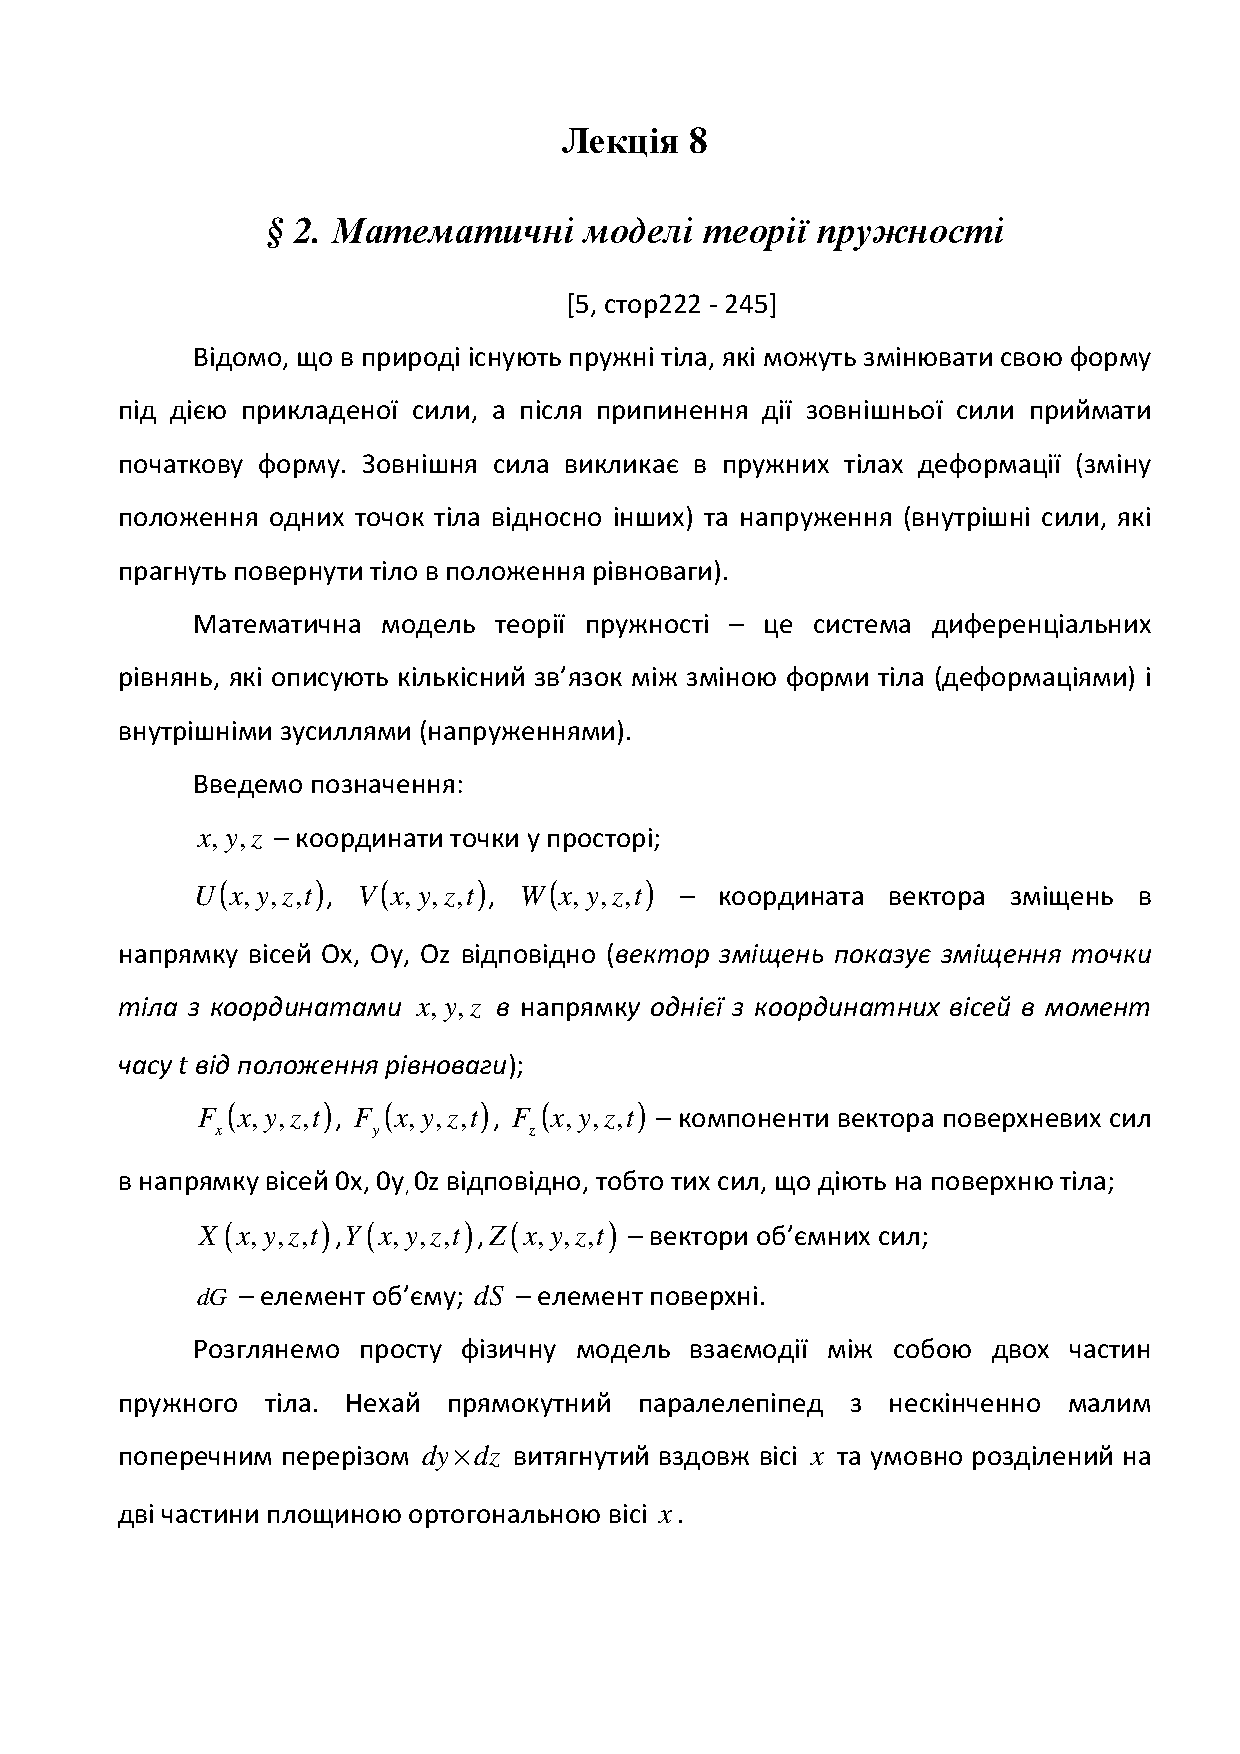
\includegraphics[]{../img/8.1}
\end{figure}

Охарактеризуємо силу з якою правий паралелепіпед діє на лівий паралелепіпед через переріз $\diff y \times \diff z$ в площині $yOz$ (на рис. площина взаємодії виділена сірим кольором). \medskip

Нехай $\bf{t}^{(x)} = \left( \sigma_x, \tau_{xy}, \tau_{xz} \right)$ --- \it{вектор сили}.

\begin{definition}[вектора сили]
	\it{Вектор сили} показує, з якою силою (на одиницю поверхні) правий паралелепіпед діє на лівий паралелепіпед.
\end{definition}

\begin{remark}
	При цьому $\sigma_x$ --- компонента, що може стискати, або розтягувати лівий паралелепіпед, $\tau_{xy}$, $\tau_{xz}$ --- компоненти, що зрізають (точне визначення цього поняття буде надано далі) паралелепіпед в напрямках вісей $Oy$ та $Oz$ відповідно.
\end{remark}

Аналогічно, для паралелепіпедів витягнутих вздовж вісей $Oy$ та $Oz$ можна розглянути сили, яки діють в двох інших площинах $xOz$ та $xOy$ на одиницю площі цих перерізів та охарактеризувати їх векторами:
\begin{align}
	\bf{t}^{(y)} &= \left( \tau_{yx}, \sigma_y, \tau_{yz} \right), \\
	\bf{t}^{(z)} &= \left( \tau_{zx}, \tau_{zy}, \sigma_z \right).
\end{align}

Для будь-якого паралелепіпеда з довжиною ребер $\diff x$, $\diff y$, $\diff z$ а тим самим точки простору напружений стан тіла можна охарактеризувати матрицею
\begin{equation}
	\label{eq:3.2.3}
	\begin{pmatrix}
		\sigma_x & \tau_{xy} & \tau_{xz} \\
		\tau_{yx} & \sigma_y & \tau_{yz} \\
		\tau_{zx} & \tau_{zy} & \sigma_z
	\end{pmatrix}
\end{equation}

\begin{remark}
	При розгляді моделі взаємодії правого паралелепіпеда та лівого паралелепіпеда через спільний переріз має місце принцип рівнодії та протидії, тобто сила, з якою правий паралелепіпед діє на лівий паралелепіпед рівна за величиною та протилежна за напрямком силі з якою лівий паралелепіпед діє на правий паралелепіпед. Сили, що діють на тіло обираються зі знаком плюс, якщо вони діють на переріз, який обмежує тіло з боку зростаючих значень координатних вісей і зі знаком мінус, якщо вони діють на поверхню, що обмежує тіло з боку спадаючих значень координатних вісей.
\end{remark}

\subsubsection{Закони рівноваги елемента поверхні}

Розглянемо елементарну модель пружної взаємодії. Нехай всередині пружного тіла ми виділили нескінченно малий тетраедр $OABC$, $\vec n$ --- вектор зовнішньої нормалі до грані $ABC$, а $S$ --- площа цієї грані:
\begin{figure}[H]
	\centering
	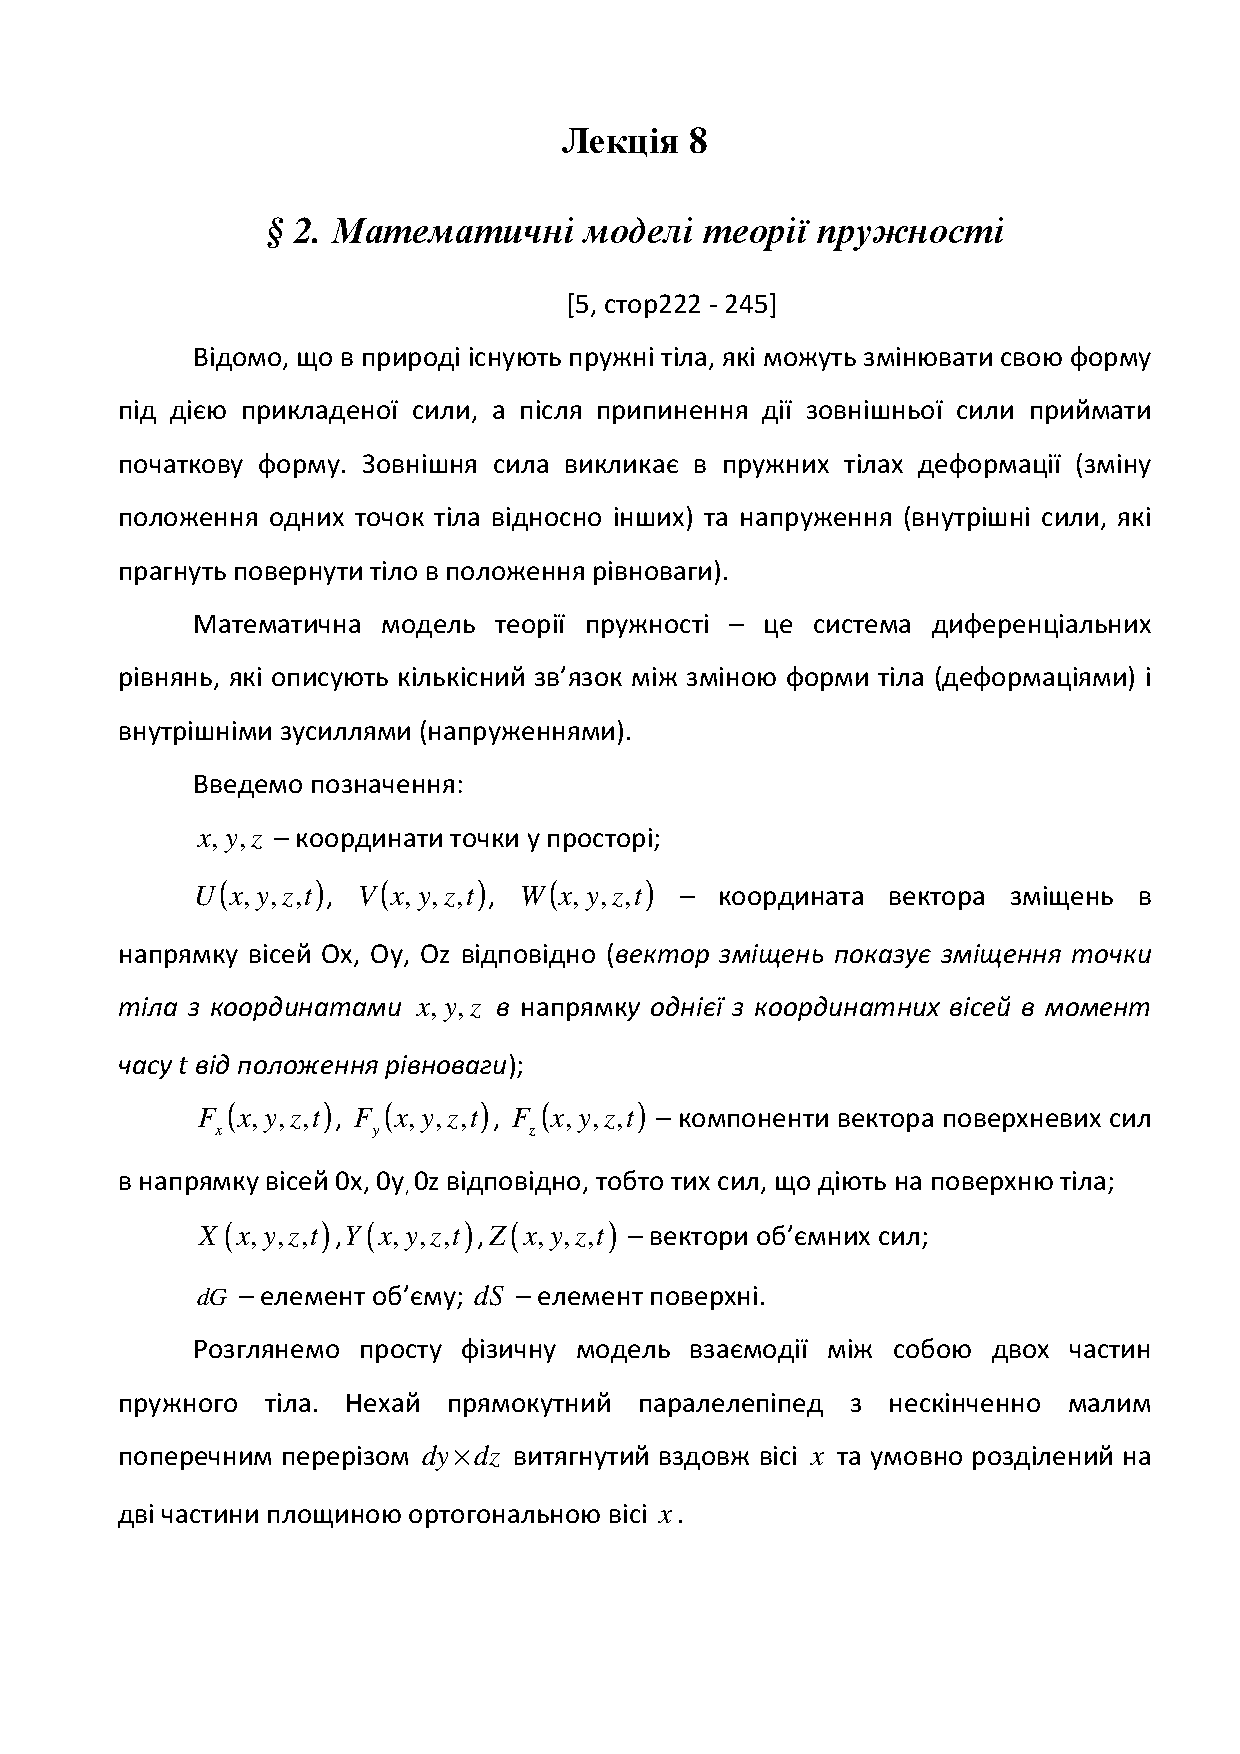
\includegraphics[]{../img/8.2}
\end{figure}

Нехай $\vec f = (f_x, f_y, f_z)$ --- вектор поверхневої сили, що діє на одиницю площі грані $ABC$. \medskip

Вектор нормалі
\begin{equation}
	\vec{\bf{n}} = \big( \cos( \vec n, x ), \cos ( \vec n, y ), \cos ( \vec n, z ) \big),
\end{equation}
а
\begin{equation}
	S \cdot \cos (\vec n, x ), \quad S \cdot \cos (\vec n, y ), \quad S \cdot \cos (\vec n, z) 	
\end{equation} 
--- площі граней тетраедра, ортогональних вісям $Ox$, $Oy$, $Oz$. \medskip

Якщо тетраедр знаходиться в стані спокою, або рівномірного прямолінійного руху, то рівнодіюча сил, що діють на всі чотири грані дорівнює нулю, тобто: 
\begin{equation}
	\vec f \cdot S - \bf{t}^{(x)} \cdot S \cdot \cos ( \vec n, x) - \bf{t}^{(y)} \cdot S \cdot \cos ( \vec n, y) - \bf{t}^{(z)} \cdot S \cdot \cos ( \vec n, z) = 0.
\end{equation}

Після скорочення на $S$ отримаємо
\begin{theorem}[векторна форма закону рівноваги елемента поверхні]
	Виконується співвідношення:
	\begin{equation}
		\vec f = \bf{t}^{(x)} \cdot \cos ( \vec n, x) + \bf{t}^{(y)} \cdot \cos ( \vec n, y) + \bf{t}^{(z)} \cdot \cos ( \vec n, z).
	\end{equation}
\end{theorem}

Запишемо закон рівноваги елемента поверхні в скалярному вигляді:
\begin{align}
	\sigma_x \cdot \cos ( \vec n, x ) + \tau_{xy} \cdot \cos ( \vec n, y ) + \tau_{xz} \cdot \cos ( \vec n, z ) &= f_x, \\
	\tau_{yx} \cdot \cos ( \vec n, x ) + \sigma_y \cdot \cos ( \vec n, y ) + \tau_{yz} \cdot \cos ( \vec n, z ) &= f_y, \\
	\tau_{zx} \cdot \cos ( \vec n, x ) + \tau_{zy} \cdot \cos ( \vec n, y ) + \sigma_z \cdot \cos ( \vec n, z ) &= f_z.
\end{align}

У випадку, коли елементарний трикутник $ABC$ є частиною реальної зовнішньої поверхні тіла, то закон рівноваги елемента поверхні приймає вигляд:
\begin{align}
	\sigma_x \cdot \cos ( \vec n, x ) + \tau_{xy} \cdot \cos ( \vec n, y ) + \tau_{xz} \cdot \cos ( \vec n, z ) &= F_x, \\
	\tau_{yx} \cdot \cos ( \vec n, x ) + \sigma_y \cdot \cos ( \vec n, y ) + \tau_{yz} \cdot \cos ( \vec n, z ) &= F_y, \\
	\tau_{zx} \cdot \cos ( \vec n, x ) + \tau_{zy} \cdot \cos ( \vec n, y ) + \sigma_z \cdot \cos ( \vec n, z ) &= F_z,
\end{align}
де $(F_x, F_y, F_z)$ --- вектор поверхневих сил. \medskip

\subsubsection{Закон рівноваги елемента об'єму}

Розглянемо будь-який об'єм $G$ обмежений поверхнею $S$ та його елементарний об'єм $\diff G$. \medskip

Об'ємні сили, що діють на тіло об'єму $G$ можна обчислити у вигляді
\begin{equation}
	\Iiint_G \begin{pmatrix} X \\ Y \\ Z \end{pmatrix} \diff G.
\end{equation}

Через будь-яку елементарну поверхню тіла діє поверхнева сила $\vec f \cdot \diff S$, а результуюча поверхнева сила, яка діє на тіло через усю поверхню $S$ має вигляд 
\begin{equation}
	\Iint_S \vec f \diff S,
\end{equation}
або, в скалярному вигляді:
\begin{equation}
	\Iint_S ( \bf{t}^{(x)} \cdot \cos ( \vec n, x ) + \bf{t}^{(y)} \cdot \cos(\vec n, y) + \bf{t}^{(z)} \cdot \cos (\vec n, z) ) \diff S.
\end{equation}

\begin{theorem}[векторний запис закону рівноваги елементу об'єму]
	Для того щоб тіло знаходилося в стані спокою або рухалось рівномірно і прямолінійно, рівнодіюча об'ємної та поверхневої сил повинна дорівнювати нулю:
	\begin{multline}
		\Iint_S \big( \bf{t}^{(x)} \cos(\vec n, x) + \bf{t}^{(y)} \cos(\vec n, y) + \bf{t}^{(z)} \cos(\vec n, z) \big) \diff S + \\ 
		+ \Iiint_G \begin{pmatrix} X \\ Y \\ Z \end{pmatrix} \diff G = 0.
	\end{multline}
\end{theorem}

\begin{theorem}[скалярний запис закону рівноваги елементу об'єму]
	\begin{system}
		\Iint_S \left( \sigma_x \cos(\vec n, x) + \tau_{yx} \cos(\vec n, y) + \tau_{zx} \cos(\vec n, z)\right) \diff S + \Iiint_G X \diff G &= 0, \\
		\Iint_S \left( \tau_{xy} \cos(\vec n, x) + \sigma_y \cos(\vec n, y) + \tau_{zy} \cos(\vec n, z)\right) \diff S + \Iiint_G Y \diff G &= 0, \\
		\Iint_S \left( \tau_{xz} \cos(\vec n, x) + \tau_{yz} \cos(\vec n, y) + \sigma_z \cos(\vec n, z)\right) \diff S + \Iiint_G Z \diff G &= 0.
	\end{system}
\end{theorem}

\begin{remark}
	Додатковою умовою рівноважного положення тіла окрім закону рівноваги елементу об'єму є виконання закону збереження моментів сил з якого випливає симетричність матриці \eqref{eq:3.2.3}:
	\begin{equation}
		\tau_{x y} = \tau_{y x}, \quad \tau_{x z} = \tau_{z x}, \quad \tau_{y z} = \tau_{z y}.
	\end{equation}
\end{remark}

Враховуючи факт симетрії, останній закон можна записати у вигляді
\begin{system}
	\Iint_S \left( \bf{t}^{(x)}, \vec n\right) \diff S + \Iiint_G X \diff G &= 0, \\
	\Iint_S \left( \bf{t}^{(y)}, \vec n\right) \diff S + \Iiint_G Y \diff G &= 0, \\
	\Iint_S \left( \bf{t}^{(z)}, \vec n\right) \diff S + \Iiint_G Z \diff G &= 0.
\end{system}
де 
\begin{equation}
	\vec{\bf{n}} = \big( \cos(\vec n, x), \cos(\vec n, y), \cos(\vec n, z) \big)
\end{equation}
--- вектор зовнішньої нормалі до поверхні. \medskip

Враховуючи формулу Остроградського-Гауса, кожен поверхневий інтеграл перетворимо в об'ємний, в результаті отримаємо
\begin{theorem}[диференціальна форма запису закону рівноваги елементу об'єму]
	Виконуються співвідношення:
	\begin{system}
		\Iiint_G \left( \nabla \cdot \bf{t}^{(x)} + X \right) \diff G &= 0, \\
		\Iiint_G \left( \nabla \cdot \bf{t}^{(y)} + Y \right) \diff G &= 0, \\
		\Iiint_G \left( \nabla \cdot \bf{t}^{(z)} + Z \right) \diff G &= 0.
	\end{system}
\end{theorem}

\begin{definition}[тензора напружень]
	В подальшому симетричну матрицю \eqref{eq:3.2.3} будемо називати \it{тензором напружень}.
\end{definition}

\subsubsection{Тензор напружень, головні вісі тензора напружень}

Позначимо через $\bf{e}_x$, $\bf{e}_y$, $\bf{e}_z$ орти прямокутної система координат з координатними осями $Ox$, $Oy$, $Oz$. \medskip 

Введемо нову систему координат з ортами $\bf{e}_\xi$, $\bf{e}_\eta$, $\bf{e}_\zeta$ та осями $O\xi$, $O\eta$, $O\zeta$. \medskip

З'ясуємо, яким чином пов'язані вектори $\bf{t}^{(x)}$, $\bf{t}^{(y)}$, $\bf{t}^{(z)}$ які складають рядки (стовпці) тензору напружень у системі координат $x$, $y$, $z$, з векторами $\bf{t}^{(\xi)}$, $\bf{t}^{(\eta)}$, $\bf{t}^{(\zeta)}$ які складають стрічки (стовпці) тензору напружень у новій системі координат $\xi$, $\eta$, $\zeta$. \medskip

Згідно до загальних формул переходу від одного ортогонального базису до іншого, можна записати:
\begin{system}
	\bf{t}^{(\xi)} &= \bf{t}^{(x)} \cdot \cos (\xi, x) + \bf{t}^{(y)} \cdot \cos (\xi, y) + \bf{t}^{(z)} \cdot \cos (\xi, z), \\
	\bf{t}^{(\eta)} &= \bf{t}^{(x)} \cdot \cos (\eta, x) + \bf{t}^{(y)} \cdot \cos (\eta, y) + \bf{t}^{(z)} \cdot \cos (\eta, z), \\
	\bf{t}^{(\zeta)} &= \bf{t}^{(x)} \cdot \cos (\zeta, x) + \bf{t}^{(y)} \cdot \cos (\zeta, y) + \bf{t}^{(z)} \cdot \cos (\zeta, z).
\end{system}

Координати ортів нової системи координат мають значення:
\begin{align}
	\bf{e}_\xi &= \big( \cos (\xi, x), \cos (\xi, y), \cos (\xi, z) \big), \\
	\bf{e}_\eta &= \big( \cos (\eta, x), \cos (\eta, y), \cos (\eta, z) \big), \\
	\bf{e}_\zeta &= \big( \cos (\zeta, x), \cos (\zeta, y), \cos (\zeta, z) \big).
\end{align}
 
Для знаходження будь-якої компоненти тензора напружень $\tau_{\alpha\beta}$, необхідно обчислити скалярний добуток
\begin{equation}
	\tau_{\alpha \beta} = \langle \bf{t}^{(\alpha)}, \bf{e}_\beta \rangle.
\end{equation}

Так, наприклад,
\begin{equation}
	\begin{aligned}
		\tau_{\xi \eta} &= \big( \sigma_x \cos (\eta, x) + \tau_{x y} \cos (\eta, y) + \tau_{x z} \cos (\eta, z) \big) \cdot \cos (\xi, x) + \\
		&\quad + \big( \tau_{y x} \cos (\eta, x) + \sigma_y \cos (\eta, y) + \tau_{y z} \cos (\eta, z) \big) \cdot \cos (\xi, y) + \\
		&\quad + \big( \tau_{z x} \cos (\eta, x) + \tau_{z y} \cos (\eta, y) + \sigma_z \cos (\eta, z) \big) \cdot \cos (\xi, z) = \\
		&= \Sum_{a, b \in \{x, y, z\}} \tau_{a b} \cos (\xi, a) \cos (\eta, b).
	\end{aligned}
\end{equation}

Отже, для довільної компоненти тензора напружень має місце 
\begin{theorem}[формула переходу до нової системи координат]
	Виконуються співвідношення вигляду
	\begin{equation}
		\tau_{\alpha \beta} = \Sum_{a, b \in \{x, y, z\}} \tau_{a b} \cos (\alpha, a) \cos (\beta, b).
	\end{equation}
\end{theorem}

\begin{remark}
	Тут використані позначення $\tau_{\alpha \alpha} = \sigma_\alpha$, $\tau_{a a} = \sigma_a$.
\end{remark}

Таким чином, тензор напружень --- це симетрична матриця
\begin{equation}
	T = 
	\begin{pmatrix}
		\sigma_x & \tau_{xy} & \tau_{xz} \\
		\tau_{yx} & \sigma_y & \tau_{yz} \\
		\tau_{zx} & \tau_{zy} & \sigma_z
	\end{pmatrix},
\end{equation}
компоненти якої перетворюються за формулою вище при переході до нової прямокутної системи координат. \medskip

Поставимо задачу вибору нової прямокутної системи координат, для якої тензор напружень має діагональну форму. Нехай $\bf{e}_{v_i}$, $i = 1, 2, 3$ --- орти нової прямокутної системи координат. Для того, щоб тензор $T$ мав діагональну форму запису, кожен вектор $\bf{t}^{(v_i)}$, $i = 1, 2, 3$ в новій системі координат повинен бути колінеарним відповідному орту $\bf{e}_{v_i}$, $i = 1, 2, 3$ тобто $\bf{t}^{(v_i)} = \sigma_i \vec v_i$. \medskip

Скористаємось формулою переходу від однієї до іншої системи координат та запишемо співвідношення для пошуку ортів:
\begin{equation}
	\bf{t}^{(v)} = \sigma \bf{e}_v = \sigma \big( \cos(v, x), \cos (v, y), \cos (v, z) \big).
\end{equation}

Запишемо останнє співвідношення в координатному вигляді:
\begin{system}
	\sigma_x \cos(v, x) + \tau_{xy} \cos(v, y) + \tau_{xz} \cos(v, z) &= \sigma \cos(v, x), \\
	\tau_{yx} \cos(v, x) + \sigma_y \cos(v, y) + \tau_{yz} \cos(v, z) &= \sigma \cos(v, y), \\
	\tau_{zx} \cos(v, x) + \tau_{zy} \cos(v, y) + \sigma_z \cos(v, z) &= \sigma \cos(v, z).
\end{system}

Для ортонормованого базису
\begin{equation}
	\cos^2(v, x) + \cos^2(v, y) + \cos^2(v, z) = 1.
\end{equation}

Тому в матрично-векторній формі попередні співвідношення мають вигляд
\begin{equation}
	T \bf{e}_v = \sigma \bf{e}_v.	
\end{equation}

Ця задача на власні значення з симетричною матрицею має три дійсних власних числа, позначимо їх $\sigma_1$, $\sigma_2$, $\sigma_3$ тобто 
\begin{equation}
	\begin{vmatrix}
		(\sigma_x - \sigma) & \tau_{y x} & \tau_{z x} \\
		\tau_{x y} & (\sigma_y - \sigma) & \tau_{z y} \\
		\tau_{x z} & \tau_{y z} & (\sigma_z - \sigma),
	\end{vmatrix} = 0
\end{equation}
і три ортонормовані власні вектори
\begin{equation}
	\bf{e}_{v_i} = \big( \cos(v_i, x), \cos(v_i, y), \cos(v_i, z) \big), \quad i = 1, 2, 3.
\end{equation}

\begin{definition}[головних вісей тензора напружень]
	Координатні вісі, для яких тензор напружень має діагональний вигляд, називаються \it{головними вісями тензора напружень}.
\end{definition}

\begin{definition}[головних компонент тензора напружень]
	Відповідні діагональні компоненти тензора напружень $\sigma_i$, $i = 1,2,3$ називаються \it{головними компонентами тензора напружень}. 
\end{definition}

Використовуючи формулу переходу між системами координат, запишемо зв'язок між компонентами тензора напружень в декартових координатах $x$, $y$, $z$ і головними компонентами тензора напружень:
\begin{align}
	\tau_{a b} &= \Sum_{i = 1}^3 \sigma_i \cos(v_i, a) \cos (v_i b), \\
	\sigma_a &= \Sum_{i = 1}^3 \sigma_i \cos^2(v_i, a),
\end{align}
де $x, b \in \{x, y, z\}$.

\subsubsection{Тензор деформацій і закони його перетворення}

Раніше були введені характеристики:

\begin{equation}
	U(x, y, z, t), \quad V(x, y, z, t), \quad W(x, y, z, t)
\end{equation}
--- зміщення точки з координатами $(x, y, z)$ від положення рівноваги в напрямку відповідної вісі. \medskip

Розглянемо можливі види деформації.
\begin{enumerate}
	\item Нормальні деформації. \smallskip

	\begin{definition}[нормальних деформацій]
		\it{Нормальні деформації} --- зміна довжини в напрямку координатної вісі --- характеризуються відносною зміною довжини відрізків.
	\end{definition}

	Приклавши силу в напрямку вісі $Ox$, точка $x$ змістилася і зайняла положення $x + U(x, \cdot, \cdot)$; точка $x + \diff x$ теж змістилася і зайняла положення $(x + \diff x) + U(x + \diff x, \cdot, \cdot)$:
	\begin{figure}[H]
		\centering
		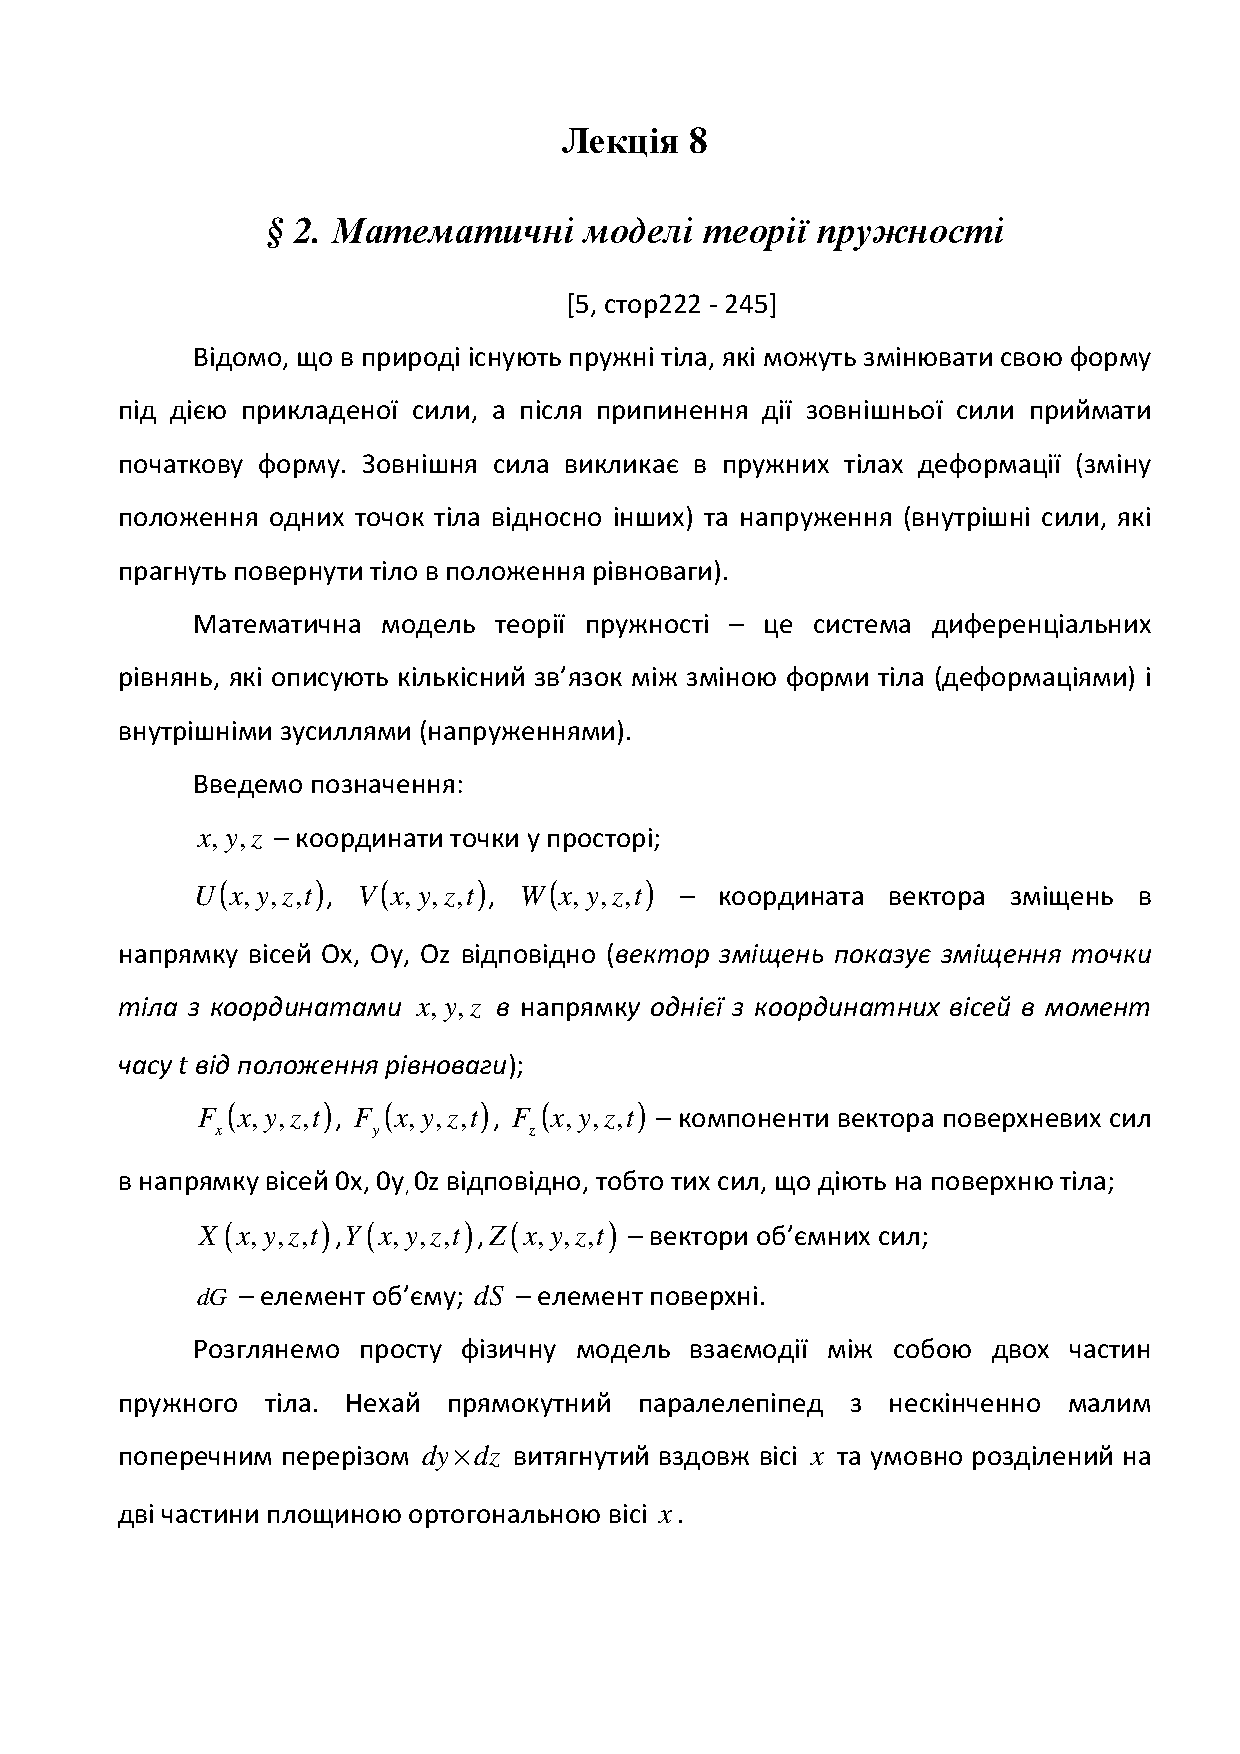
\includegraphics[]{../img/8.3}
	\end{figure}

	Порахуємо відносне подовження відрізка $\diff x$ після прикладення до нього напруження:
	\begin{multline}
		\frac{(x + \diff x) + U(x + \diff x, \cdot, \cdot) - x - U(x, \cdot, \cdot) - \diff x}{\diff x} = \\
		= \frac{U(x + \diff x, \cdot, \cdot) - U(x, \cdot, \cdot)}{\diff x} \xrightarrow[\diff x \to 0]{} \frac{\partial U}{\partial x}.
	\end{multline}

	Аналогічно, можна ввести характеристику відносного подовження в напрямку двох інших вісей. \medskip

	Отже, нормальні деформації характеризуються частинними похідними
	\begin{equation}
		\frac{\partial U}{\partial x}, \quad \frac{\partial V}{\partial y}, \quad \frac{\partial W}{\partial z}.
	\end{equation}

	\item Зрізаючі (дотичні) деформації. \smallskip

	\begin{definition}[зрізаючих (дотичних) деформацій] 
		\it{Зрізаючі (дотичні) деформації} будемо характеризувати абсолютною зміною кутів між відрізками в кожній з трьох координатних площин, які до початку дії напружень були ортогональними.
	\end{definition}

	Розглянемо фізичну модель зрізуючих деформацій. Нехай відрізки $AB$ та $CD$ довжини $\diff x$ та $\diff y$  відповідно після дії прикладених сил зайняли положення $A' B'$ та $C' D'$ відповідно:
	\begin{figure}[H]
		\centering
		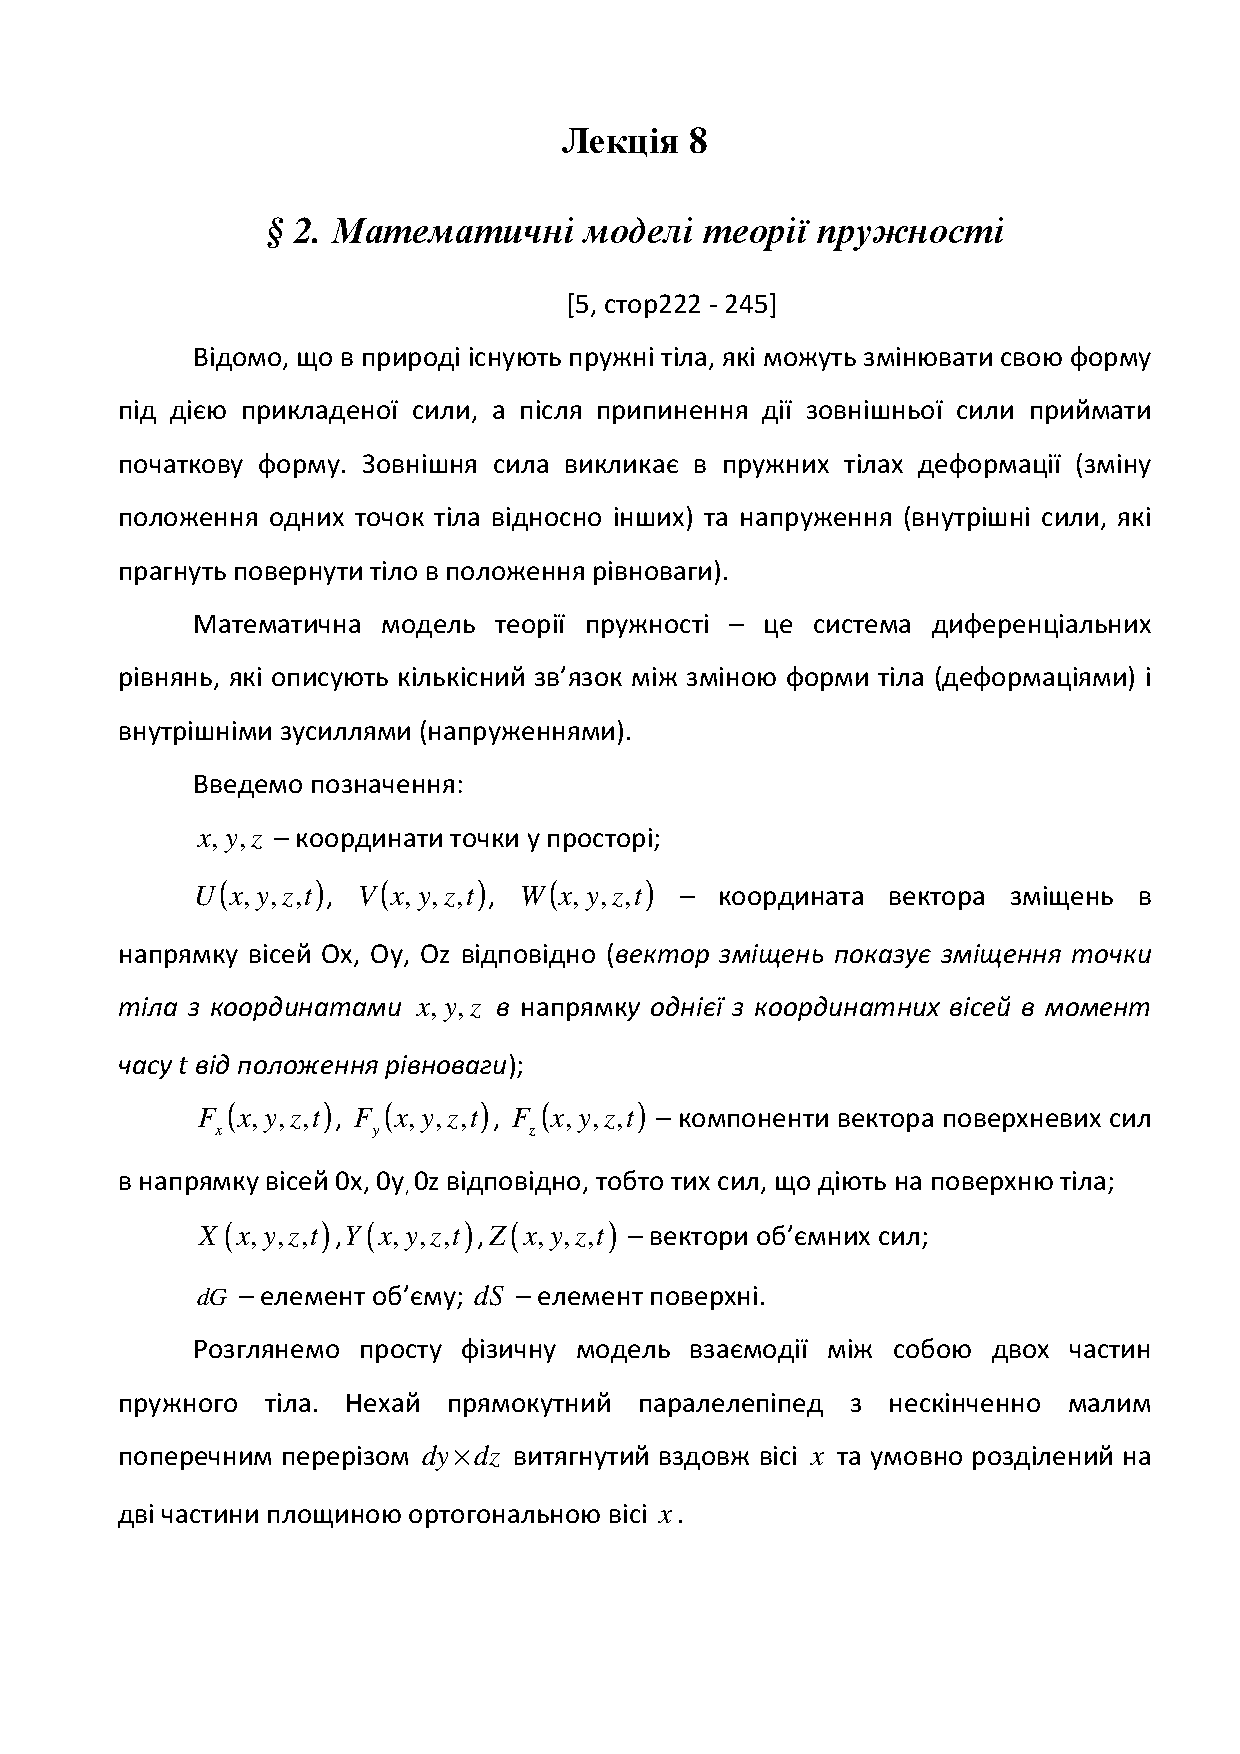
\includegraphics[]{../img/8.4}
	\end{figure}

	Точка $A$ змістилася на відстань $V(x, \cdot, \cdot)$, а точка $B$ змістилася на відстань $V(x + \diff x, \cdot, \cdot)$. \medskip

	Тоді
	\begin{equation}
		\frac{V(x + \diff x, \cdot, \cdot) -V(x, \cdot, \cdot)}{\diff x} = \tan \alpha \xrightarrow[\diff x \to 0]{} \frac{\partial V}{\partial x},
	\end{equation}
	тому
	\begin{equation}
		\alpha \approx \tan \alpha = \partial V / \partial x.
	\end{equation}

	Аналогічно $\beta \approx \partial U / \partial y$. \medskip

	Сумарна зміна кута
	\begin{equation}
		\alpha + \beta \approx \frac{\partial V}{\partial x} + \frac{\partial U}{\partial y}.
	\end{equation}
	
	Позначимо
	\begin{equation}
		\gamma_{x y} = \frac{\partial V}{\partial x} + \frac{\partial U}{\partial y} = \gamma_{y x}.
	\end{equation}
	
	Провівши аналогічні міркування щодо інших координатних площин отримаємо: 
	\begin{align}
		\gamma_{x z} &= \frac{\partial W}{\partial x} + \frac{\partial U}{\partial z} = \gamma_{z x}, \\
		\gamma_{y z} &= \frac{\partial W}{\partial y} + \frac{\partial V}{\partial z} = \gamma_{z y}.
	\end{align}

	Позначимо також
	\begin{equation}
		\epsilon_x = \frac{\partial U}{\partial x}, \quad \epsilon_y = \frac{\partial V}{\partial y}, \quad \epsilon_z = \frac{\partial W}{\partial z},
	\end{equation}
	і $\gamma_{a a} = 2 \epsilon_a$. \medskip

	В результаті повну деформацію у будь-якій точці простору можна охарактеризувати 
	\begin{definition}[тензора деформацій]
		Симетрична матриця
		\begin{equation}
			\begin{pmatrix}
				\epsilon_x & \gamma_{x y} & \gamma_{x z} \\
				\gamma_{y x} & \epsilon_y & \gamma_{y z} \\
				\gamma_{z x} & \gamma_{z y} & \epsilon_z
			\end{pmatrix}
		\end{equation}
		називається симетричним \it{тензором деформацій}.
	\end{definition}
\end{enumerate}

\subsubsection{Перетворення тензора деформацій до нових прямокутних координат}

Вивчимо перетворення симетричного тензору деформацій при переході від однієї прямокутної системи координат до іншої. Нехай $O\xi$, $O\eta$, $O\zeta$ --- вісі нової системи координат (замість $Ox$, $Oy$, $Oz$), а функції $U'$, $V'$, $W'$ --- зміщення в напряму нових вісей. \medskip

Враховуючи формули переходу від одного ортогонального базису до іншого можемо записати:
\begin{system}
	U' &= U \cos (\xi, x) + V \cos (\xi, y) + W \cos (\xi, z), \\
	V' &= U \cos (\eta, x) + V \cos (\eta, y) + W \cos (\eta, z), \\
	W' &= U \cos (\zeta, x) + V \cos (\zeta, y) + W \cos (\zeta, z),
\end{system}
а також
\begin{system}
	x &= \xi \cos (\xi, x) + \eta \cos (\eta, x) + \zeta \cos (\zeta, x), \\
	y &= \xi \cos (\xi, y) + \eta \cos (\eta, y) + \zeta \cos (\zeta, y), \\
	z &= \xi \cos (\xi, z) + \eta \cos (\eta, z) + \zeta \cos (\zeta, z),
\end{system}
і
\begin{system}
	\xi &= x \cos (\xi, x) + y \cos (\xi, y) + z \cos (\xi, z), \\
	\eta &= x \cos (\eta, x) + y \cos (\eta, y) + z \cos (\eta, z), \\
	\zeta &= x \cos (\zeta, x) + y \cos (\zeta, y) + z \cos (\zeta, z).
\end{system}
 
У цих формулах 
\begin{equation}
	\big( \cos (\alpha, x), \cos (\alpha, y), \cos (\alpha, z) \big) = \bf{e}_\alpha, \quad \alpha \in \{\xi, \eta, \zeta\}.
\end{equation}
--- координати ортів нового базису. \medskip

Знайдемо вирази для компонентів тензору у новій системі координатах: $\epsilon_\alpha$, $\gamma_{\alpha, \beta}$ при $\alpha, \beta \in \{\xi, \eta, \zeta\}$. \medskip

Зокрема для $\epsilon_\xi$ отримаємо:
\begin{equation}
	\begin{aligned}
		\epsilon_\xi &= \frac{\partial U'}{\partial x} = \left( \frac{\partial U}{\partial x} \frac{\partial x}{\partial \xi} + \frac{\partial U}{\partial y} \frac{\partial y}{\partial \xi} + \frac{\partial U}{\partial z} \frac{\partial z}{\partial \xi}\right) \cos (\xi, x) + \\
		& \quad + \left( \frac{\partial V}{\partial x} \frac{\partial x}{\partial \xi} + \frac{\partial V}{\partial y} \frac{\partial y}{\partial \xi} + \frac{\partial V}{\partial z} \frac{\partial z}{\partial \xi}\right) \cos (\xi, y) + \\
		& \quad + \left( \frac{\partial W}{\partial x} \frac{\partial x}{\partial \xi} + \frac{\partial W}{\partial y} \frac{\partial y}{\partial \xi} + \frac{\partial W}{\partial z} \frac{\partial z}{\partial \xi}\right) \cos (\xi, z) = \\
		&= \cos (\xi, x) \left( \frac{\partial U}{\partial x} \cos (\xi, x) + \frac{\partial U}{\partial y} \cos (\xi, y) + \frac{\partial U}{\partial z} \cos (\xi, z)\right) + \\
		&\quad + \cos (\xi, y) \left( \frac{\partial V}{\partial x} \cos (\xi, x) + \frac{\partial V}{\partial y} \cos (\xi, y) + \frac{\partial V}{\partial z} \cos (\xi, z)\right) + \\
		&\quad + \cos (\xi, z) \left( \frac{\partial W}{\partial x} \cos (\xi, x) + \frac{\partial W}{\partial y} \cos (\xi, y) + \frac{\partial W}{\partial z} \cos (\xi, z)\right).
	\end{aligned}
\end{equation}
     
Розкриваючи дужки і використовуючи відповідні позначення отримаємо наступну формулу:
\begin{equation}
	\gamma_{\xi \xi} = 2 \epsilon_\xi  = \Sum_{a, b \in \{x, y, z\}} \gamma_{a b} \cos (\xi, a) \cos(\xi b).
\end{equation}

Отже у загальному вигляді доведена
\begin{theorem}[формула перетворення тензора деформацій]
	Виконуються співвідношення вигляду:
	\begin{equation}
		\gamma_{\alpha \beta} = \Sum_{a, b \in \{x, y, z\}} \gamma_{a b} \cos (\alpha, a) \cos(\beta b),
	\end{equation}
	де $\alpha, \beta \in \{\xi, \eta, \zeta\}$.
\end{theorem}

\end{document}